\section{Experiment 2}
This experiment investigates the effects of pattern recognition in higher dimensional domains. In order to do this the training error would now be regenerated for every new dimension considered (5, 10, 15), but would remain constant in that loop. The test dataset, however, would be regenerated on every iteration of the experiment. Once again following a similar format to the training cycle and repetitions as in Experiment 1, this experiment also has one fundamental difference in that since the training error will effectively remain constant (relative to the dimension). However the testing error should approach the true error value which was approximated by the $E(500)$ error probability approximation. As instructed the covariance matrix was selected to be an identity matrix, and the class means were designed in a way that $\mu_{1}$ is a random vector of integers, and that $\mu_{2}$ is offset by a random fractional distance from $\mu_{1}$. The weights were manually adjusted to ensure that the error probability value remained within the range of 5-10\% for all dimensions.

\subsection{Results \& Discussion}
Unlike the expected convergence, the errors were seen to oscillate prior to convergence. This oscillation was more present at lower values of $N_{D}$ and convergence to reasonable performance needed larger training datasets in lower dimensions. As seen in Figure \ref{fig:exp2-a} the oscillation lasts longer in the 5 dimensional space as opposed to the 10 and 15 dimensional spaces as seen in Figure \ref{fig:exp2-b}. Though these experiments were conducted in low granularity it's clear that between 100-200 training sample sets are needed at a higher dimension of 10 or 15. 

\begin{figure}[H]
	\centering
	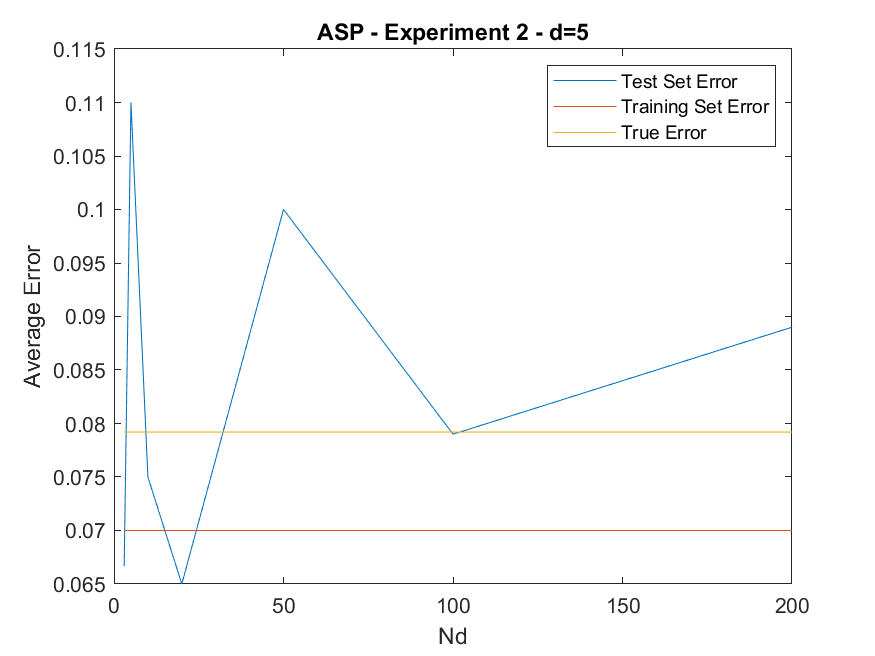
\includegraphics[width=.8\linewidth]{./code/Exp2-results/ErrorComparison_5.png}
	\caption{5 Dimensions}
	\label{fig:exp2-a}
\end{figure}

\begin{figure}[h]
	\centering
	\begin{subfigure}{.5\textwidth}
		\centering
		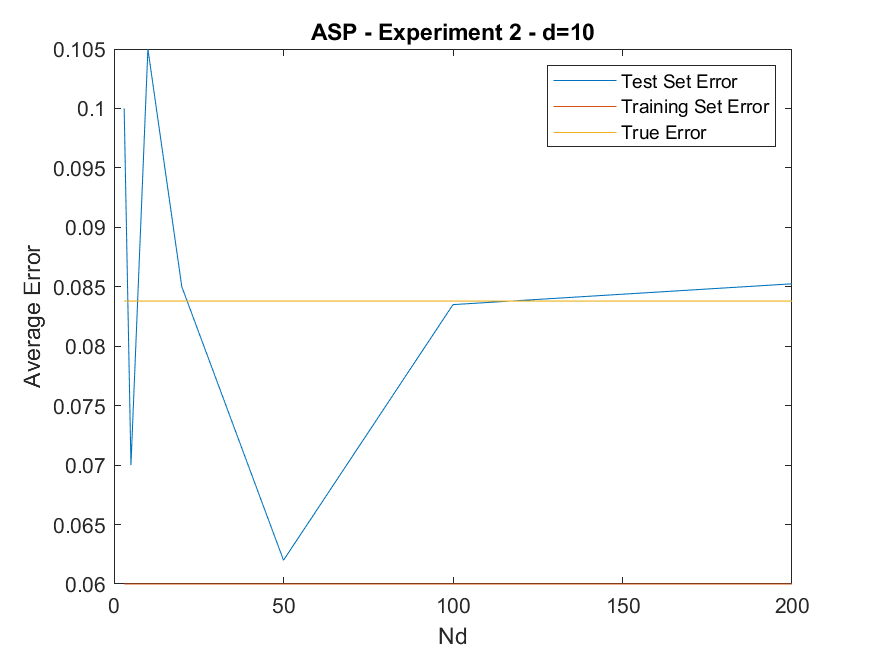
\includegraphics[width=.95\linewidth]{./code/Exp2-results/ErrorComparison_10.png}
		\caption{10 Dimensions}
	\end{subfigure}%
	\begin{subfigure}{.5\textwidth}
		\centering
		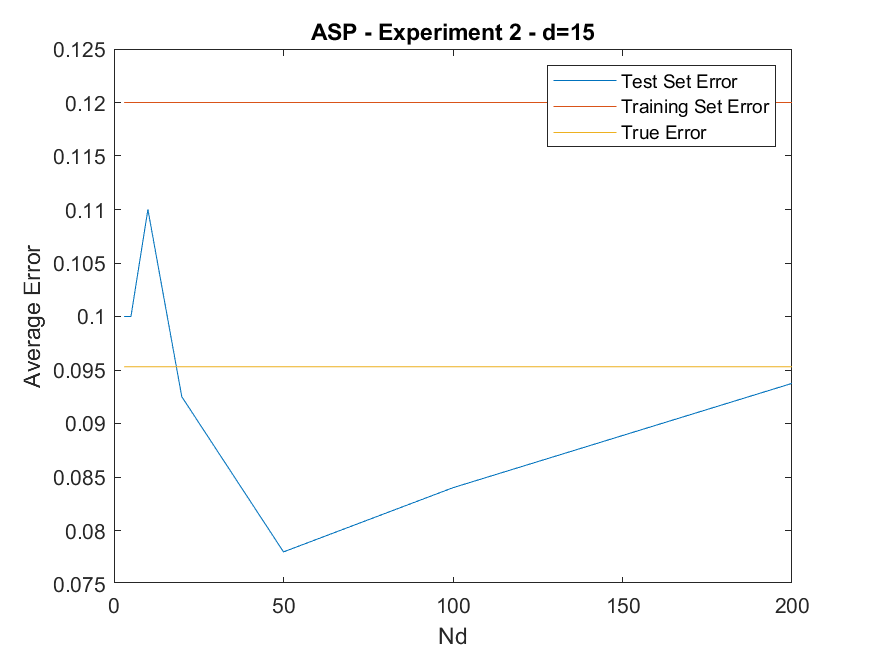
\includegraphics[width=.95\linewidth]{./code/Exp2-results/ErrorComparison_15.png}
		\caption{15 Dimensions}
	\end{subfigure}
	\caption{Experiment 2 Results - Mean Error Comparison vs Test Set Size}
	\label{fig:exp2-b}
\end{figure}
